\chapter{Graphics Processing Units} \label{chapter:graphics_processing_units}

In this work, we aim to accelerate the execution of our solver using a relatively new architecture,
GPUs. GPUs are massively parallel computer chips that have recently started to be used in the
scientific computing domain. GPUs have initially been used to compute graphical computations, such
as the output to a computer screen, video processing, and synthetic image generation. These
computations are \textit{embarrassingly parallel}, meaning that they are comprised of many identical
computations independent of each other. GPUs are therefore optimised for parallel efficiency.
Combined with the fact that these problems deal with huge amounts of data, GPUs are also optimised
for maximum bandwidth. They are significantly different from \textit{Central Processing Units
(CPUs)}, the traditional architecture on which code is run. CPUs are optimised to solve serial
problems as fast as possible, meaning the prioritise serial speed over parallel efficiency, and
latency over bandwidth. 

Solving fluid flows over a mesh is a parallel problem, as at most steps it is possible to compute
the solution on the different elements making up the mesh in parallel. On the other hand, elements
must exchange information at their interfaces at each time step, meaning careful synchronisation
will be needed. Finally, the adaptivity process detailed in
Chapter~\ref{chapter:adaptive_mesh_refinement} and the load balancing process from
Chapter~\ref{chapter:load_balancing} are not inherently parallel processes. A lot of effort will
have put into breaking up these algorithms into parallel tasks to be run on GPUs. Overall, if it is
possible to efficiently parallelise these sequential parts of the problem, the gains from running
the main solving loop on the highly parallel GPUs should incur a significant speedup to the program.

\section{Architecture} \label{section:graphics_processing_units:architecture}
% Start by saying each GPU has an associated CPU
% Talk about treads and blocks
% thread warps, branching
% Talk about saturation, SEMs
% How it doesn't work well with adaptivity usually
% Again sequential vs parallel, with high clock, cache and control flow vs lower clock, more
% processing power, more smaller cores
% GPUs have CPUs
% Concurrent execution

\begin{figure}[H]
	\centering
	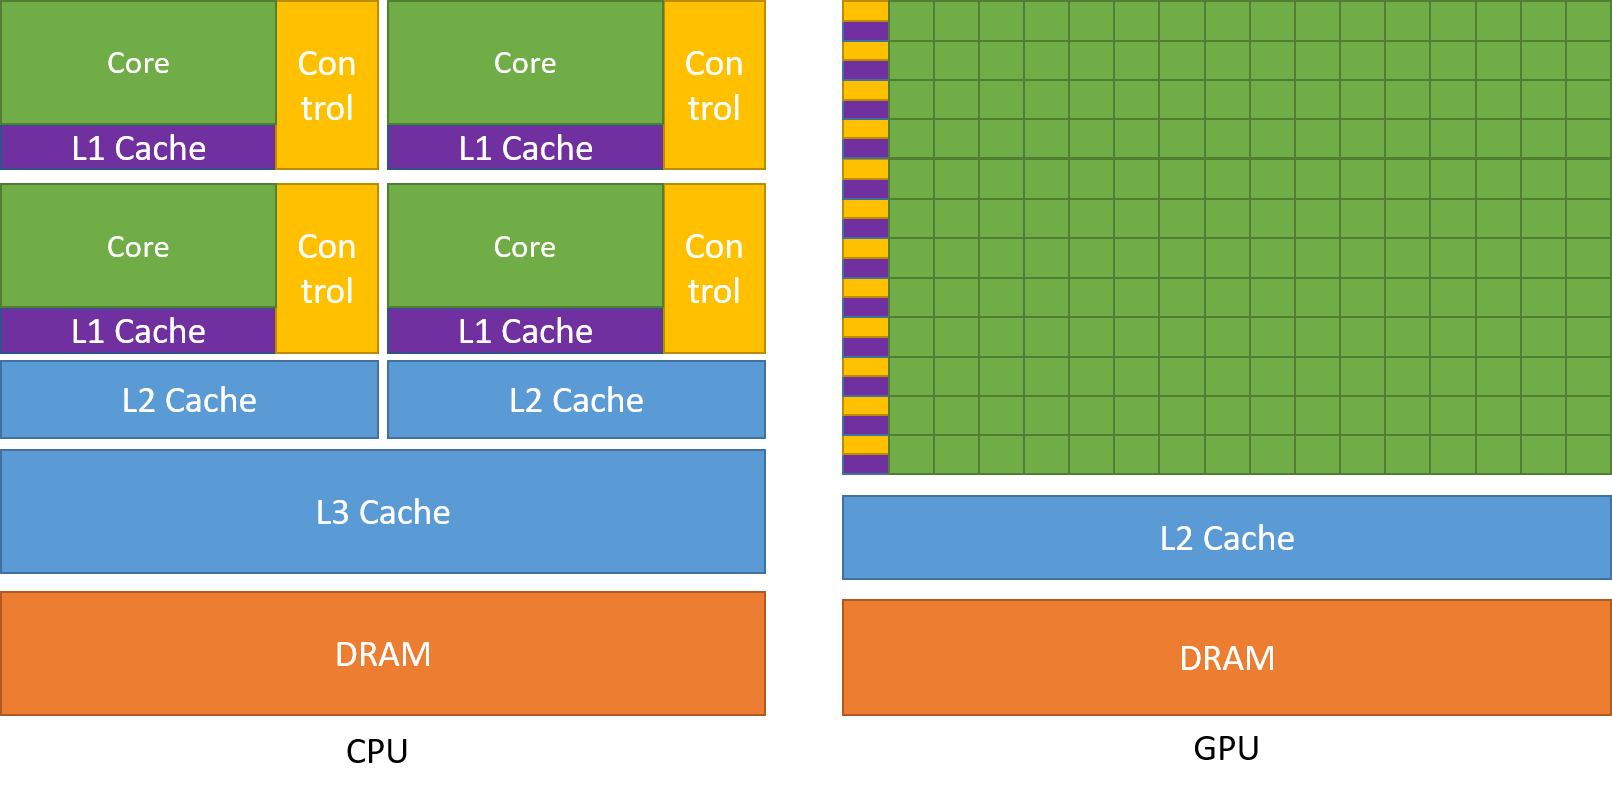
\includegraphics[width=0.8\textwidth]{Chapter_graphics_processing_units/media/gpu-devotes-more-transistors-to-data-processing}
	\caption{CPU and GPU architecture: GPUs dedicate more space to data processing}
	\label{fig:cpu_gpu}
\end{figure}

Graphics processing units and central processing units are fundamentally made up of the same core
components. First, data processing hardware is shown in green. These are the parts of the chips that
do calculations on data. Then, in yellow is control flow. Control flow hardware schedules
instructions to be executed on processing hardware. In orange is the main memory of either
architecture. Main memory stores data to be used for computations. It is very big, and takes
relatively long to access. Finally, in blue and purple is different levels of cache. Cache is much
smaller and much faster than main memory, and as such stores parts of the memory that the processing
hardware is actively using in order to speed up access.

The two architectures differ as to the balance between the size and capacities of those components.
Chip area is limited by the processes used to manufacture them, so the different components must
share this limited spaces, and sacrifices must be made. GPUs dedicate much more space to data
processing. 

\begin{figure}[H]
	\centering
	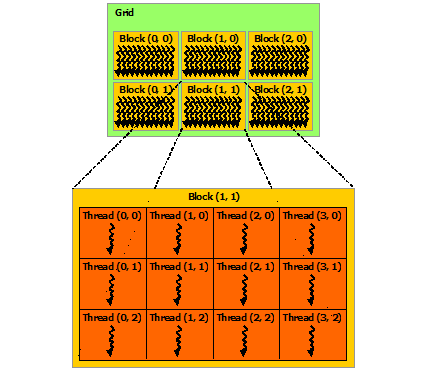
\includegraphics[width=0.6\textwidth]{Chapter_graphics_processing_units/media/grid-of-thread-blocks}
	\caption{GPU programming model: Execution is split into multiple parallelism levels}
	\label{fig:gpu_programming_model}
\end{figure}

\section{Data structure} \label{section:graphics_processing_units:data_structure}
% Mesh design, unstructured
% Talk about dynamic memory
% Talk about data structure? The fact we use unstructured meshes, are the worse case for GPU
% Talk about how data is allocated
% Race conditions, when information is exchanged (ex fluxes)

\section{Process Parallelism} \label{section:graphics_processing_units:process_parallelism}
% GPU partitions
% Say something about worker processes, to be general with cpu workers.

When trying to solve very large problems, a single node with a single GPU will have insufficient
processing power and memory to solve the problem in a reasonable time, or at all. To work with these
larger problems, the work needs to be split at another level than GPU parallelism.  

The program can use multi-block meshes, with each block being worked on by one process and one GPU.
If there are fewer GPUs available on a system than there are processes, some processes will share a
single GPU by using asynchronous execution streams. The different processes communicate together
using \textit{Message Passing Interface (MPI)} at their boundaries. Since the solution data resides
on the GPU, it must first be copied to the main CPU memory before it is sent through the MPI
runtime. It then needs to be copied to the receiving process' GPU. This exchange necessitates
multiple transfers on different levels and should be optimised as much as possible. An approach to
minimise the number of interfaces between the different mesh blocks is explained in
Chapter~\ref{chapter:load_balancing}. 

\section{Implementation} \label{section:graphics_processing_units:implementation}
% Talk about reductions
% Talk about kernels
% Talk about reduce operations, data transfers for boundaries
